\documentclass{acm_proc_article-sp}
\usepackage{listings}
\usepackage{amsmath} % For "split" math environment.
\hyphenation{data-base}
\lstset{language=SQL}

\begin{document}
\title{Share*Match: EECS341 Project}
\subtitle{Final Project Report}
\numberofauthors{3}
\author{
\alignauthor Ian Dimayuga \\
    \email{ian.dimayuga@case.edu}\\
\alignauthor Tom Dooner \\
    \email{tom.dooner@case.edu}\\
\alignauthor Brian Stack \\
    \email{brian.stack@case.edu}
}
\maketitle
\begin{abstract}
We have developed a simple web application which uses a relational database to permit users to share items that would otherwise go unutilized in their own homes.  The project was built using modern web development practices including RESTful interfaces, AJAX interactions, MVC architecture, and testing. 
\end{abstract}

\section{Introduction}
% From Project Proposal 1
In the world of homeownership, it is often necessary to purchase items which are not regularly used. 
Unfortunately, these items, once purchased, often lie on shelves for months unused. 
Meanwhile, neighbors or close friends may require similar items and may purchase these items themselves if they didn't think to ask those who live around them.

ShareMatch seeks to meet this need. We have built a web application that leverages the locality of users to 
enable local connection to save money. By having users log in and be able to search for local items that fit 
their criteria, users can save money on purchasing those items for one-off uses. And, if a user happens to own 
an unusual device, he or she can list the device on the site where others can find it.

To aid this process, we will build a sort of \textit{sharing karma} system that is based on trust. 
By having users trust their real-life friends, we can prioritize search requests as well as provide 
users visual feedback of a user's real-life responsibility and likelihood to return items.

\section{Application Requirements Specification}
% From Project Proposal 1
When a user navigates to the ShareMatch homepage, he or she should see a page with pictures of items on it.
This serves to give the user an indication of what types of items have recently been shared or are new items posted. 
Clicking on an image of an item should bring the user to the page for that item upon which they can opt to borrow that item if it's available.

At the top of the homepage, user management links will allow people to interact with the site in a personal way. 
A ``Register'' link will take a person to another page. The registration page will be a simple page with multiple 
text fields for properties of a user, such as name, e-mail address, and password. After completing the registration, the new user will be informed that they can now log in with their e-mail address and password.

The top of the homepage will also contain a link to allow users to log in. In typical UI design, after clicking this link, the user will be presented with a box for their e-mail address and password. Clicking Login will validate their e-mail address and password, and, on correct entry, redirect them to a personalized landing page.

From the user landing page, logged-in users should be able to select their location. This will probably be implemented by a zip-code selection box. Upon entering their zip code, users will be ``joining'' the location and be sent to the location page.
On this location page, various local information will be displayed. For instance, we will show some available items in the given region along with some recently borrowed items. Naturally there will also be a list of users on this page, and clicking on their names will take you to that user's profile page. Overall, a location (ZIP code) is sort of the hub that you can go to find an item if the search method isn't working.

Upon clicking on a user's name, the browsing user will be taken to the profile page for the clicked user. A user's profile page will contain such things as a list of items that they are borrowing or have recently borrowed. Also, on the user profile page, if you are logged in, you will see a button to signify that you ``Trust'' the person.

``Trust'' is our friendship mechanism. Roughly analogous to Twitter's ''follow'', ``trust'' indicates that you want to prioritize this person's items. Items from trusted loaners will show up higher when searched for.

On a user's own profile page, the same fields show up with the addition of a button which signifies ``offer an item to loan''. Upon clicking this page, the loaning user will be taken to a page with a few fields on it regarding the item. Example fields include a Title, a short Description, some picture uploads, and some other item data. For example, one pertinent item attribute we plan to include is a desired rental time period (for instance ``I only want to loan my punching bag out for two week segments'').

Items will be categorized into tagged categories. Upon uploading an item, the uploading user can specify a list of tags which apply to that item (e.g. ``Fitness, Boxing''). Items will leverage this ontology in search pages and on user profile pages so that users can find most efficiently their desired item.

In general, users will probably find an item via our built-in search mechanism. A large box on top of most pages will invite users to input a keyword which will be matched against item names, tags, and descriptions. The most relevant items will be returned, and the items will be ranked using a combination of trustworthiness (if you trust the other user) and keyword relevance.

The search results page will be a listed display of item images. The images will be supplemented with some other information about each item. Each item image will be clickable and take the user to a page where the user can easily request to borrow that item.

On the borrowing page, the item will be displayed along with some other data about an item. For example, on Amazon (and other e-commerce sites), users may review items to provide valuable feedback. We see this paradigm as especially important for applications like this -- so that the bad items may be avoided and the better items chosen where such options exist.

Logistically, we plan to send e-mails automatically when items are requested to be borrowed. However, we also plan to implement a basic messaging system which can be used for inter-personal communication for things such as ``Oops, I broke your item.'' In this case, we
intend to implement functionality which will allow users to follow through a slightly-more-formal process to note their problem. So, users will be able to reply, forgive, or compensate to problem reports regarding their items. When possible, problem reports will appear in the normal message stream between users.

\section{Database Requirements Specification}
% From Project Proposal 1
The name is assumed to be of the standard western format of ``first last'' for the time being, although an upgrade to international standards could be made if it were necessary. Their physical address is stored because our application interacts with the real world and we need to know this for exchange of items. The email address and join date are included for obvious reasons. Finally the password hash is a necessity to allow users to log in to the site, and be authenticated as themselves.

The item table is of a similar magnitude, containing fields for value, description, date added, and maximum loan time. The first fields are fairly self explanatory, but the maximum loan time has an interesting application in that it will be used to warn users who have borrowed an item that they are heading towards the end of their allocated time. It also has a foreign key linking it to the owner of the item.

The second way that items and users are linked is through the borrowing join table. It contains the foreign keys of both users and items, with an entry indicating that the user has at some point borrowed the item. There are starting and ending dates to show for how long the user had the item, and a foreign key for an issue.

The issue table will be used to keep track of the state of a complaint against the user who borrowed or is lending the item. An example use case for this is that if the borrower breaks the item, they will notify the lender of this, and then it can be resolved through this. It contains keys for conversations that occur between the users in order to resolve the conflict.

The conversations are a major part of our application. They are also non-trivial although we have designed a system for them that is rather simple. All conversations are ongoing and take place between two users. There is no end to a conversation, and new ones do not begin later. This allows us to have a single message table that contains the primary keys of two users, in addition to the body of the message itself and a time of creation.

The conversation will be used in two ways. Primarily as a way for the lender and borrower to decide how they will exchange their items. Also as mentioned above, they will be used in conflict resolution when an issue occurs with a borrowing event.

An important foundation of our platform is the idea of trust between users. In order to support trustworthy users and identify non-trustworthy ones, we have implemented a simple system that is roughly analogous to ``friending'' on popular social networking sites. Users can trust one another, which must be reciprocated in order to take effect. When two users trust each other, their items will show up higher in any search for an item. Conversely, a user can block another user if they find them to be not worth borrowing or lending to, and then the blockee will not show up in any search blocker, and the blocker will not show up in any search by the blockee. This relationship is not reciprocal.

This relationship will be represented by a karma table that maps users onto users and has a single value that indicates whether the relation is a block or a trust. This is a flexible solution, and will be able to grow with the application over time.

One of the other most important elements of our application is the idea of tags. Each item can be tagged with some sort of text. The relationship is many to many, and is a way of enabling users to navigate the site more easily and for administrators to see what common categories of items are. It will be implemented as a simple table with a join table between items and tags.

In addition there is a simple table that will represent media of the item. This will allow users to upload images or video of the item in question. This table will merely contain a link to a url, not the actual binary blob of data. This is because web servers are very good at serving static files and can handle this much more efficiently than piping the data out of the database.

There is a table that exists for the purpose of aggregating users from similar locations. It is based on zipcode and will be used to find users who are near to each other in order to facilitate lending. It also has a description for the location and the time that the location first joined the community.

Finally, we have a system for reviews that contain a body of text and a foreign key for the user who posted the review. The nice part about these reviews is that they can be considered helpful or not helpful by other users, thereby creating a system where only useful comments are displayed at the top. This is implemented with a join table between users and comments.

There will be a set of queries that occur far more frequently than others, and so the application should be optimized towards these.

Primarily the actions associated with finding and displaying items will be run the most. This will necessitate selecting items from the items table. The results will be paginated so that more than 20 results don't have to be loaded every time this action occurs. In addition when an item is viewed a lot of things will need to be loaded and displayed. This means that there will be a lot of queries to comments tables and images or other media. In addition the table that checks to see if something is borrowed will be hit pretty hard.

The most important integrity constraint is that when a user ceases to exist, their items must be removed along with them. When a user deletes themselves, their comments will still exist, but just from an anonymous user. Also, when a user ceases to exist, his or her messages with others must remain intact along with all of the records of loaned or borrowed items.

\section{ER Model Data Design}
% From Project Proposal 2
Our ER Model Diagram is attached at the end of this document as Figure \ref{fig:ERDiagram}.
\begin{figure*}[p]
    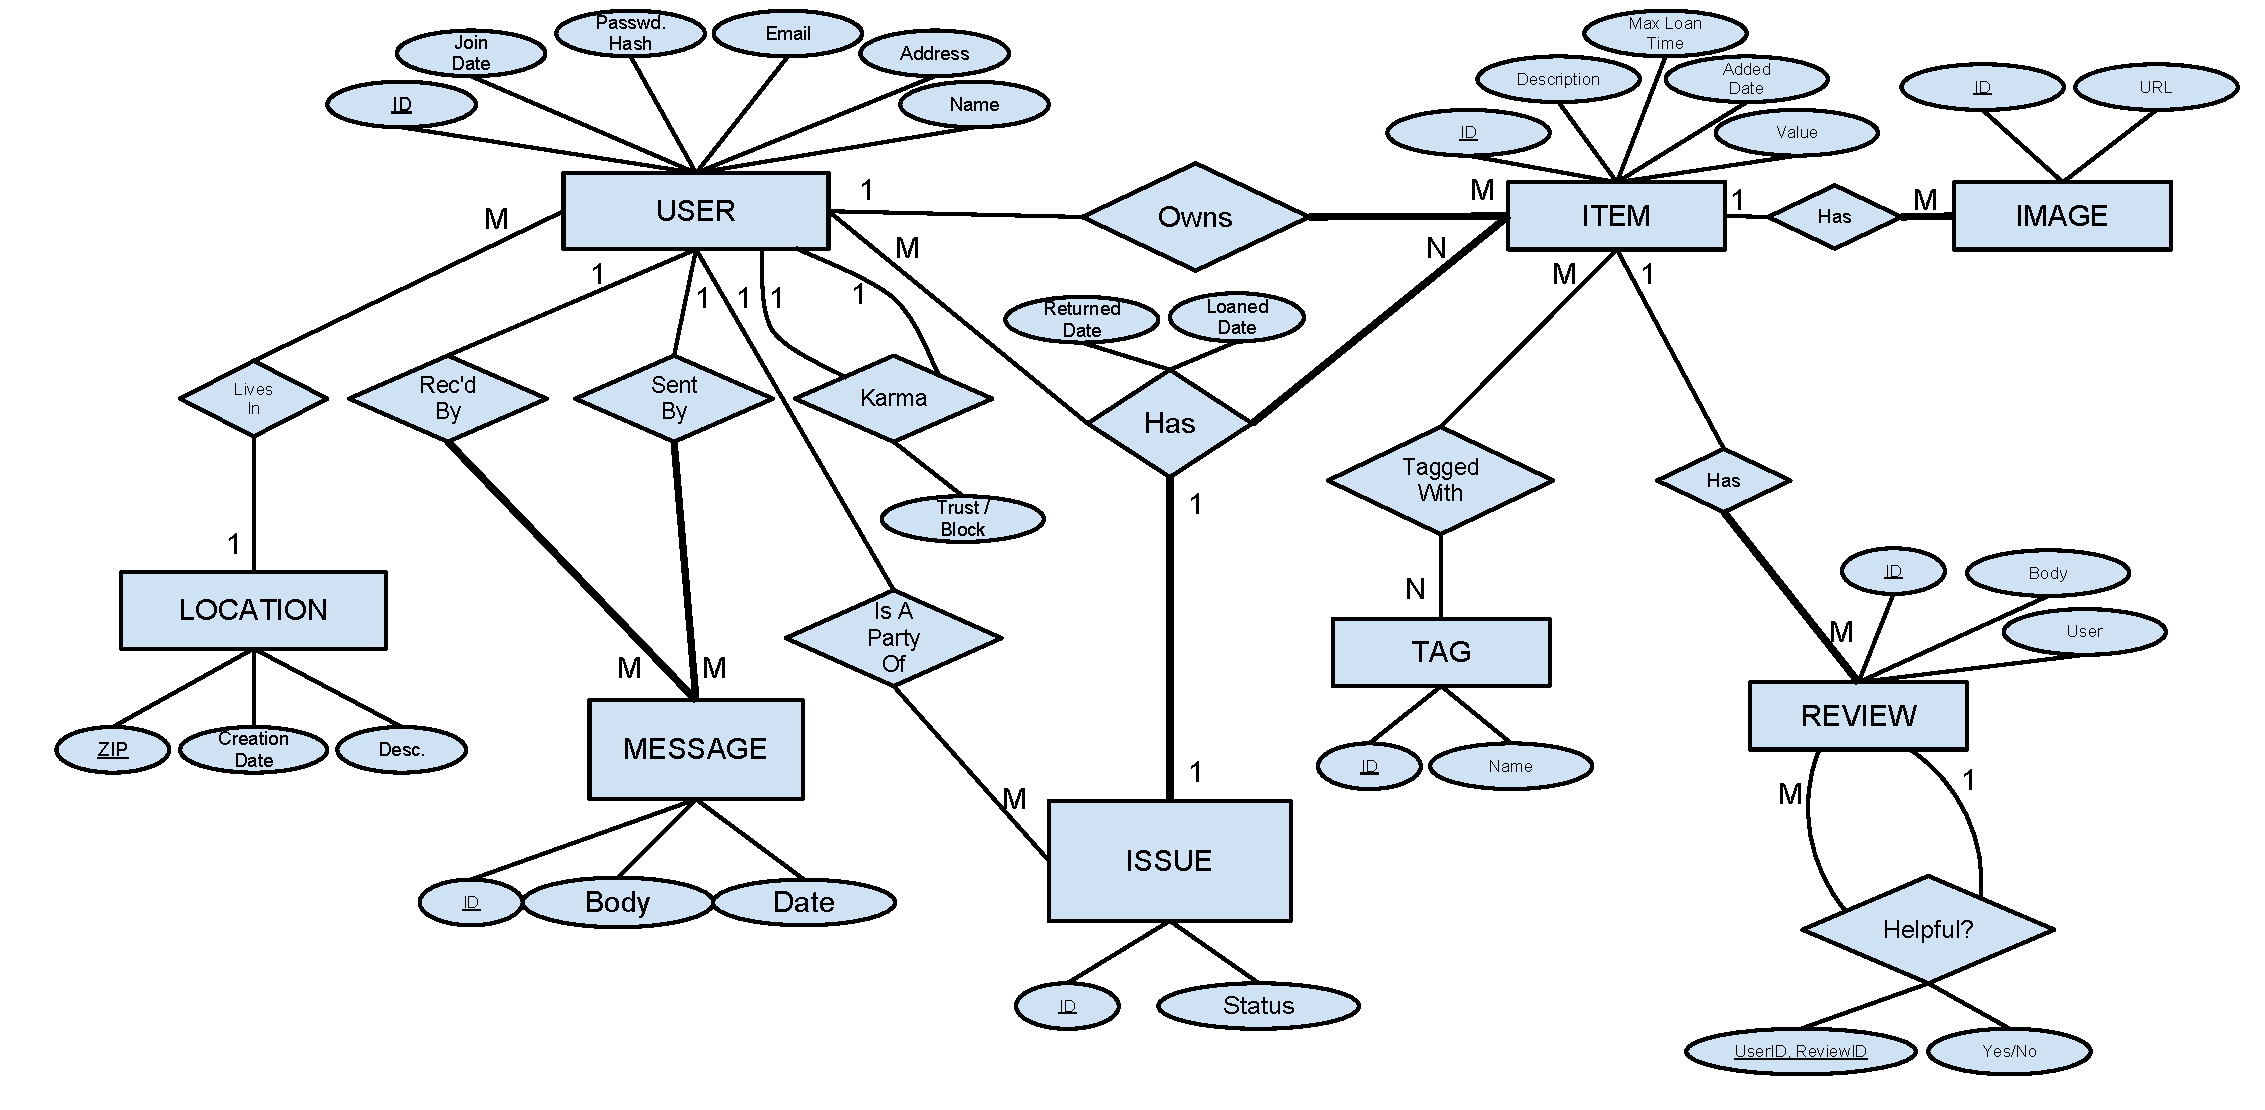
\includegraphics[width=\textwidth]{EECS341ProjectERDiagram.pdf}
    \caption{ER Diagram for Share*Match}
    \label{fig:ERDiagram}
\end{figure*}

\section{Transforming ER Model to Relational Model}
Because our ER Model was well-designed with foresight into the Relational Model, the transformation from ER to Relational was relatively straightforward. The first step was to create a table for each entity in the ER model, including their regular attributes. Second, entities with one-to-one relationships are easily joined.

Next, we handled the one-to-many relationships. In the ER Model, these are shown with relationships intermediating the one-to-many idea. This is more simply done in the Relational model with a composition. For example, each User has many Items, but each Item only has one User. Thus, we can simply assign each record in the Items table to have a User attribute, referencing the one User that owns the Item.

The many-to-many relationships were handled with join tables to represent the relationships. For example, each Item has multiple Tags, and each Tag has many Items. Therefore, we created a table Taggings, where each Tagging represents an Item and a Tag.

A different relationship involved Messages. Each message is sent from one User to another User. Thus, it can be viewed as a one-to-one join of Users, or alternatively a two-to-many relationship with Users and Messages. Regardless, we chose to have a Messages table that had one attribute for each User.
% From Project Proposal 2
Our Relational Model Diagram is attached at the end of this document as Figure \ref{fig:RelationalDiagram}.
\begin{figure*}[p]
    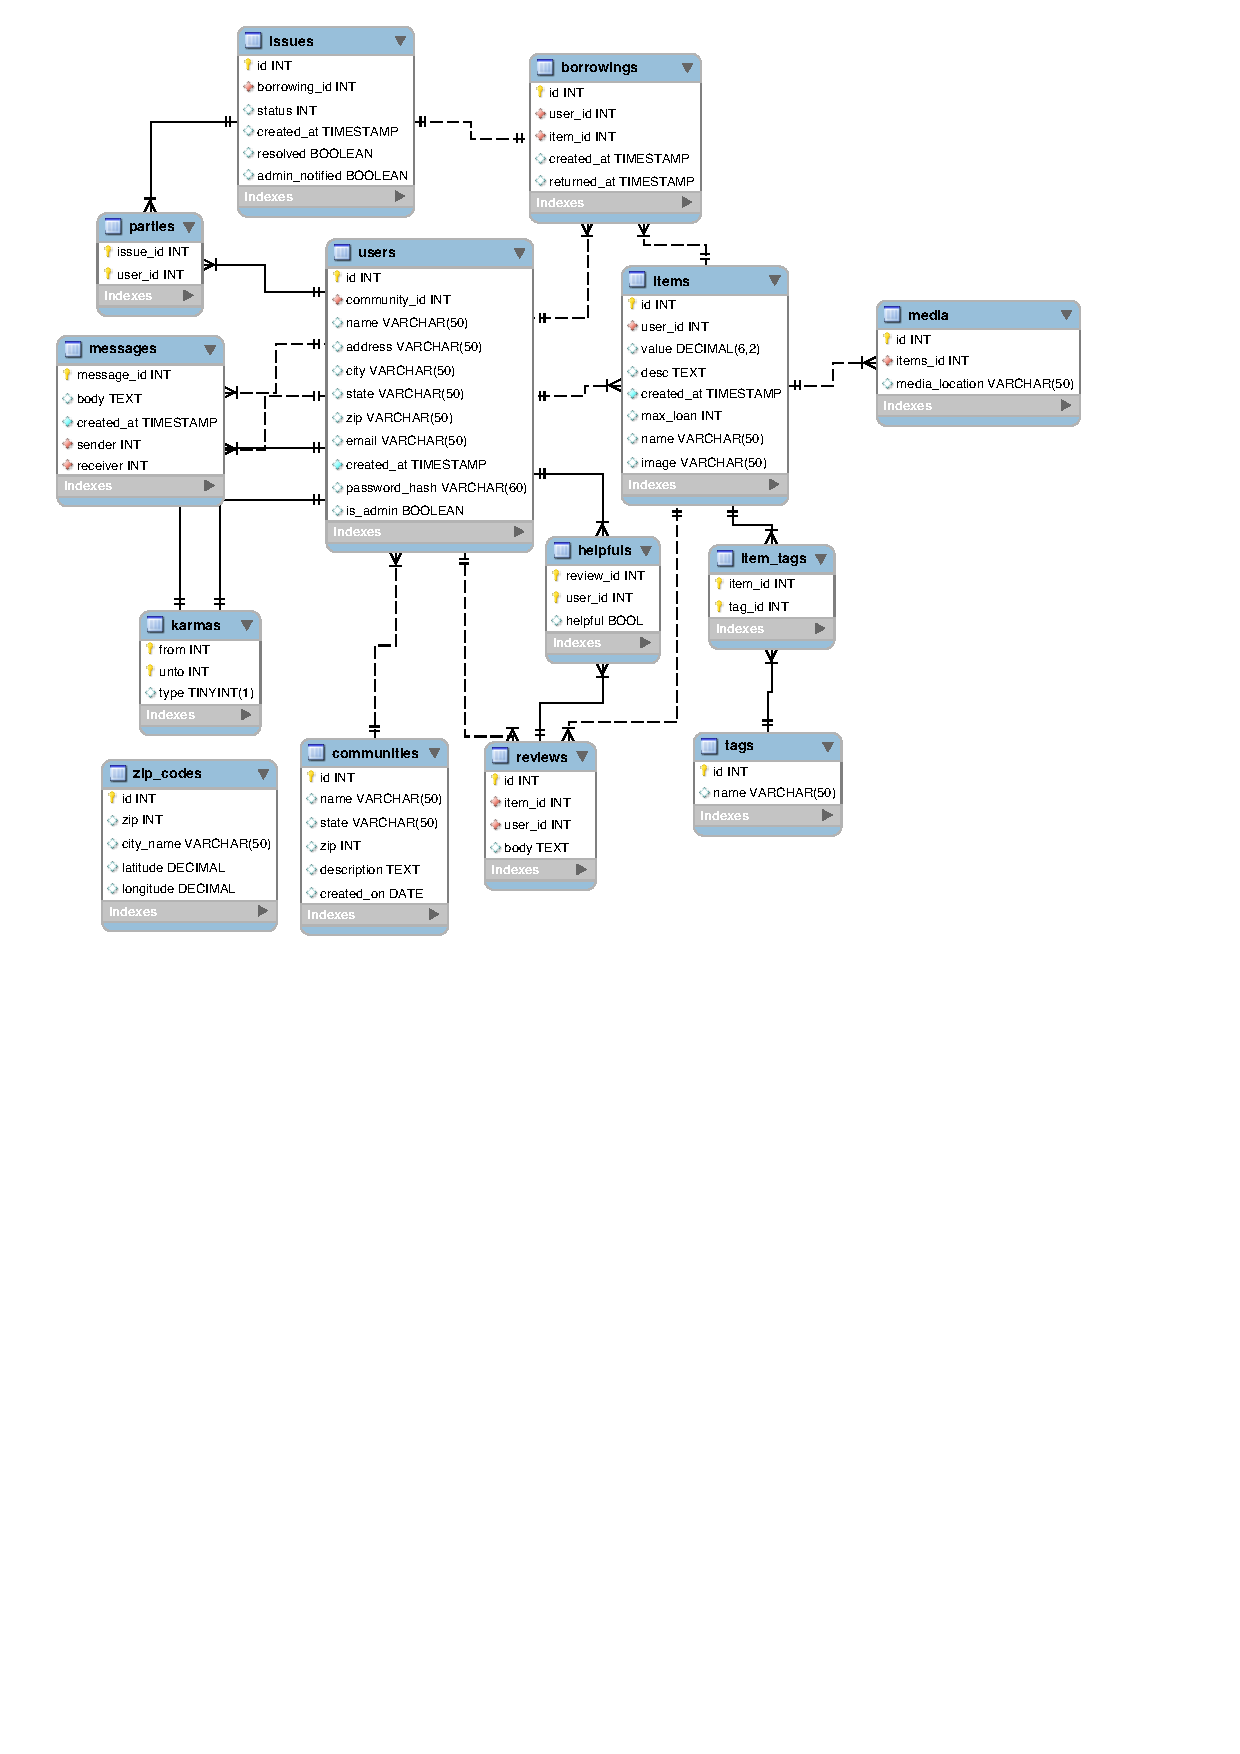
\includegraphics[width=\textwidth]{EECS341Relational.pdf}
    \caption{Relational Diagram for Share*Match}
    \label{fig:RelationalDiagram}
\end{figure*}

\section{Creating Our Database}
% From Project Proposal 3
Our SQL Create Table commands are listed at the end of this document as Figure \ref{fig:SQLCreateCommands}.
\begin{figure*}[p]
    \begin{lstlisting}
    CREATE TABLE borrowings (id INTEGER NOT NULL PRIMARY KEY AUTOINCREMENT, 
      created_at TIMESTAMP, returned_at TIMESTAMP, 
      current BOOLEAN DEFAULT 't', user_id INTEGER NOT NULL, 
      item_id INTEGER NOT NULL);

    CREATE TABLE communities (id INTEGER NOT NULL PRIMARY KEY AUTOINCREMENT,
      name VARCHAR(50), state VARCHAR(50), zip INTEGER, description TEXT, 
      created_on DATE);

    CREATE TABLE helpfuls (review_id INTEGER NOT NULL, user_id INTEGER 
      NOT NULL, helpful BOOLEAN, PRIMARY KEY(review_id, user_id));

    CREATE TABLE issues (id INTEGER NOT NULL PRIMARY KEY AUTOINCREMENT, 
      created_at TIMESTAMP, resolved BOOLEAN DEFAULT 'f', 
      admin_notified BOOLEAN DEFAULT 'f', borrowing_id INTEGER NOT NULL);

    CREATE TABLE items (id INTEGER NOT NULL PRIMARY KEY AUTOINCREMENT, 
      value DECIMAL(6, 2), created_at TIMESTAMP, max_loan INTEGER, 
      name VARCHAR(50), desc TEXT, image VARCHAR(50), 
      user_id INTEGER NOT NULL);

    CREATE TABLE item_tags (item_id INTEGER NOT NULL, 
      tag_id INTEGER NOT NULL, PRIMARY KEY(item_id, tag_id));

    CREATE TABLE karmas (from INTEGER NOT NULL, unto INTEGER NOT NULL, 
      type BOOLEAN, PRIMARY KEY(from, unto));

    CREATE TABLE locations (zip_code INTEGER NOT NULL, description TEXT, 
        created_on DATE, PRIMARY KEY(zip_code));

    CREATE TABLE messages (message_id INTEGER NOT NULL PRIMARY KEY AUTOINCREMENT, 
      body TEXT, created_at TIMESTAMP, sender_id INTEGER, receiver_id INTEGER);

    CREATE TABLE parties (issue_id INTEGER NOT NULL, user_id INTEGER 
        NOT NULL, PRIMARY KEY(issue_id, user_id));

    CREATE TABLE reviews (id INTEGER NOT NULL PRIMARY KEY AUTOINCREMENT, 
      body TEXT, created_at TIMESTAMP, user_id INTEGER NOT NULL, 
      item_id INTEGER NOT NULL);

    CREATE TABLE tags (tag_id INTEGER NOT NULL PRIMARY KEY AUTOINCREMENT, 
        name VARCHAR(50));

    CREATE TABLE users (id INTEGER NOT NULL PRIMARY KEY AUTOINCREMENT, 
      name VARCHAR(50), address VARCHAR(50), city VARCHAR(50), 
      state VARCHAR(50), zip VARCHAR(50), location_id INTEGER, 
      email VARCHAR(50), created_at TIMESTAMP, password_hash VARCHAR(60), 
      is_admin BOOLEAN, community_id INTEGER);

    CREATE TABLE zip_codes (id INTEGER PRIMARY KEY AUTOINCREMENT, 
      zip INTEGER, city_name VARCHAR(50), latitude DECIMAL, longitude DECIMAL);
    \end{lstlisting}
    \caption{SQL CREATE Commands}
    \label{fig:SQLCreateCommands}
\end{figure*}

\section{SQL Queries in RA and TRC}
By and large, as with any web application, our project consists of mostly simple queries. 
\begin{centering}
\begin{lstlisting}
SELECT * FROM items;
\end{lstlisting}
\end{centering}

As a result of using an ORM (Object-Relational Mapper), simple queries are abstracted away. 
For instance, on the ``Items with Tag'' page we wish to select all properties of
all items with a certain tag, but we do not have to write the SQL query manually. If we did, it would look something
like
\lstset{language=SQL}
\begin{lstlisting}
SELECT i.* FROM items i, taggings g, tags t 
  WHERE i.id=g.item_id AND t.tag_id=g.tag_id 
  AND t.name = ?;
\end{lstlisting}

In Relational Algebra, this query can be represented as
\[ \pi_{items.*}(\sigma_{tags.name=?}(\text{items}\bowtie\text{taggings}\bowtie\text{tags})) \]
In Tuple Relational Calculus, this query looks like (defining $I(x)$ to be tuples $x \in \textit{items}$,
$G(x)$ to be all tuples $x \in \textit{taggings}$, and $T(x)$ to be all tuples $x \in \textit{tags}$).
\begin{displaymath}
\begin{split} 
\{i | I(i) \to ((\forall g)(G(g) \to i[id] = g[item\_id] \\
\land ((\forall t)(T(t) \to g[tag\_id] = t[tag\_id] \land \\
t[name] = ?))))\}
\end{split}
\end{displaymath}

Consider also the task of finding a review by a certain user\_id for a certain item\_id. This is also
accomplished easily with the use of the ORM. Internally, the query run is equivalent to:
\begin{lstlisting}
SELECT * FROM reviews 
  WHERE item_id=? AND user_id = ?
\end{lstlisting}
Or, in Relational Algebra,
\[ \sigma_{item\_id=? \land user\_id=?}(\textit{items}) \]
Or, in Tuple-Relational Calculus (defining $R(x)$ to be true if $x$ is in the relation \textit{reviews}),
\[ \{ t | R(t) \to (t[item\_id]=? \land t[user\_id]=?) \]

However, not all queries are abstracted by the ORM. For instance, the logic to select the closest
communities to a ZIP Codes uses a table matching the ZIP Code of each community with the latitude and
longitude of that point, and then sorting by the difference in latitude and longitude.

The query from our codebase is:
\begin{lstlisting}
SELECT c.id, z.latitude, z.longitude, 
 z.latitude-(SELECT latitude 
    FROM zip_codes where zip = ?) as latdiff, 
 z.longitude-(SELECT longitude 
    FROM zip_codes where zip = ?) as londiff 
 FROM zip_codes z, communities c 
 WHERE c.zip = z.zip 
 ORDER BY latdiff*latdiff+londiff*londiff ASC;
\end{lstlisting}

In Relational Algebra and Tuple Relational Calculus, the query is actually quite simple due to the lack of order
\[ \pi_{c.id,z.latitude,z.longitude}(\textit{community}\bowtie\textit{zip\_codes}) \]
\[ 
\begin{split}\{ t | t[1] = c[id] \land t[2] = z[latitude] \land t[3] = z[longitude] \land \\
(\forall c\forall z)((C(c) \land Z(z)) \to c[zip] = z[zip])
\}
\end{split}
\]
(assuming $C(x)$ is true for tuples $x \in \textit{community}$ and $Z(x)$ is true for tuples $x \in \textit{zip\_codes}$).
%TODO: Add two more queries to this section.
% Tom's other query
Another interesting query in the Karma section is getting a list of all trusted users. This allows the find page
to intelligently prioritize the items found according to the users' preferences. The query looks something like
\begin{lstlisting}
SELECT i.* FROM items i, karmas k 
  WHERE i.user_id = k.unto AND k.from = ? AND k.type = TRUE;
\end{lstlisting}

In Relational Algebra, this can be represented as
\[ \begin{split}
\pi_{i.*}(\sigma_{k.type=TRUE \land k.from=?}( \\
  items \bowtie_{items.user\_id=karmas.unto} karmas))
\end{split}\]

In Tuple Relational Calculus, this can be represented as
\[ 
\begin{split} \{ t | I(t) \to ((\forall k) (K(k) \to t[user\_id] = k[unto] \\
\land k[from] = ? \land k[type] = TRUE)) \} \end{split} \]
\section{Integrity Constraints}
In our application, we decided to do application-level data validation as much as possible. Thus, the database
contains few constraints. For example, in our Create Table commands (in Figure \ref{fig:SQLCreateCommands}) only
the primary keys are specified to be NOT NULL. We use no stored procedures or triggers.

In the application logic, our ORM verifies a few things throughout the code -- for instance that email addresses 
are not duplicated and that certain fields are not empty. To do this, we used validations built into the ORM as
well as custom ones to ensure special constraints held. For instance, the logic to ensure an item is not borrowed
twice simultaneously is a custom validator in the Item model.
\section{Relational Database Design}
We designed our database to contain as few functional dependcies as possible. We used the standard practice of an
auto-increment primary key integer to keep otherwise-similar tuples distinct. And, since we don't store redundant information
in any table, no columns are functionally determined by any other columns.

One notable exception exists, however. In the users relation, we store a few properties including the user's city, state, and ZIP code. 
Technically, the ZIP code functionally determines both the city and the state, however we store the values in the table
anyway because they are inputted by the user, would require an additional look-up if not stored there, and are highly unlikely
to change any time soon. 

If we were to decompose the relation so that it is strictly in BCNF, we could eliminate city and state from the users
relation and create a new relation consisting of ZIP Code (primary key), city, and state.
\section{Revisiting the Relational Database Schema}
\section{DBMS Implementation}
We used SQLite version 3 as the backend database. In a serious production environment, we would probably use
a more serious DBMS such as PostgreSQL. However, SQLite provided us a portable, zero-configuration DBMS library
which supports enough of SQL to be completely usable\footnote{Interestingly, SQLite does not support the DROP COLUMN ability.}.
On the backend of our application, we used the DataMapper ruby gem to provide us an abstracted interface to
interact with the database. DataMapper uses the definitions of models to generate the structure for the database.
Also, DataMapper was built with modularity in mind, so we exploited this to include functionality such as validations,
pagination, and migrations.

One issue that we worked around was the fact that we never got into a database upgrading groove. Instead of actually
using migrations, we simply destroyed and rebuilt the database whenever the schema changed. This data loss was mitigated
by the creation of a database seeding script which automatically populates the database with lots of fake data and some
consistent user credentials for testing.

\section{Application Implementation}
\subsection{Signing Up}
Application development proceeded smoothly. Before long, we had implemented a simple web application with login functionality.
From there, we focused on producing a polished product. Figure \ref{fig:SignUpPage.png} demonstrates the log-in process
complete with frontend and backend user input validation.
\begin{figure}[h]
\begin{centering}
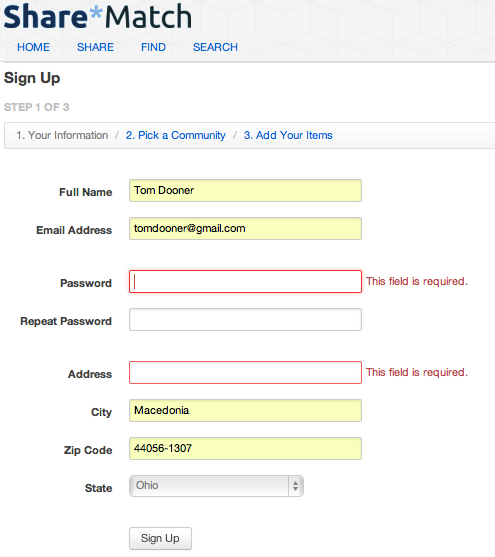
\includegraphics[width=0.4\textwidth]{SignUpPage.png} %& 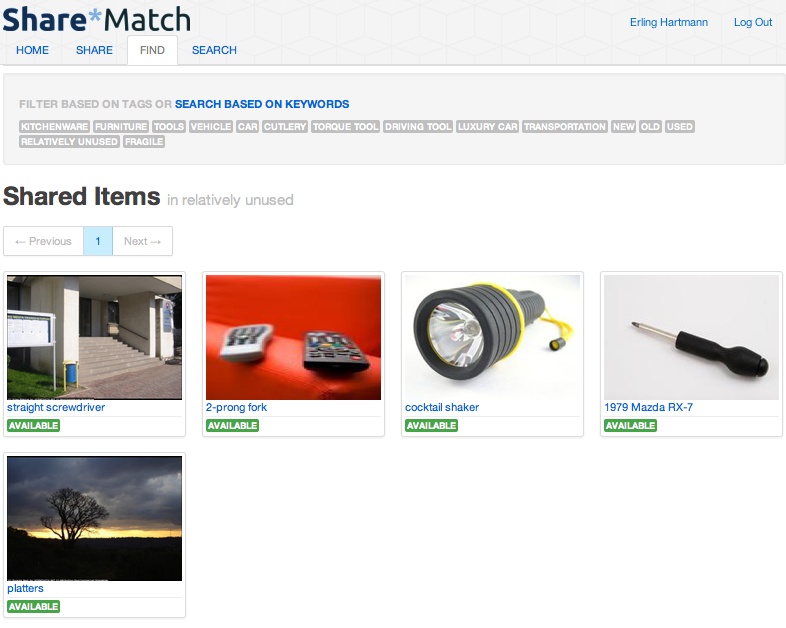
\includegraphics[width=0.25\textwidth]{ItemSearch.png} & 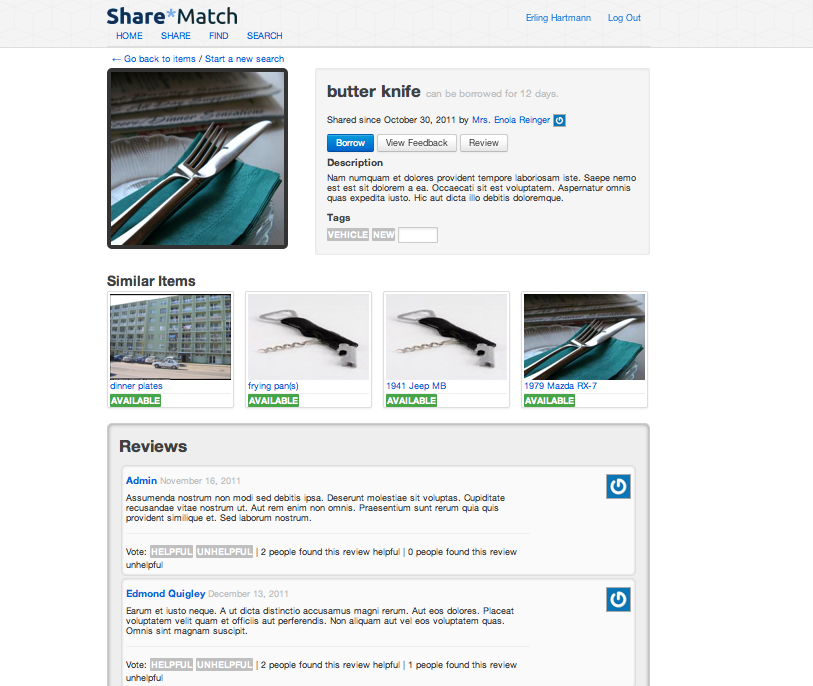
\includegraphics[width=0.25\textwidth]{ItemView.png}
\caption{The Sign Up Page}
\label{fig:SignUpPage.png}
\end{centering}
\end{figure}

\subsection{Item Finding}
From there, we focused on developing the core functionality of our application -- item sharing. A crucial aspect of borrowing
an item is the ability to find it. Hence, we built out a tagging functionality which allows users to impose a natural
categorization on items, and filter using the categorization later. Figure \ref{fig:ItemSearch.png} shows the item find
process. The grey bubbles up top are tags which allow the user to filter the results.
\begin{figure}[h]
\begin{centering}
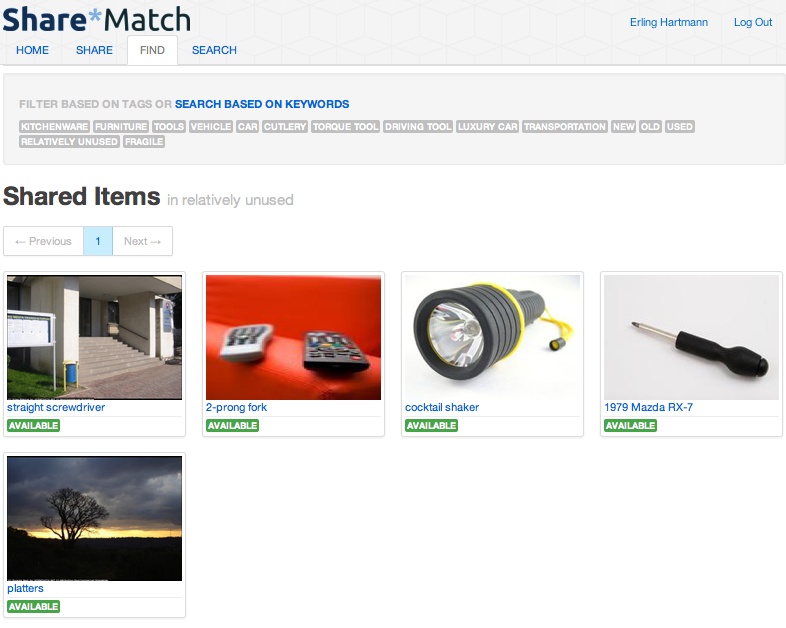
\includegraphics[width=0.4\textwidth]{ItemSearch.png}
\caption{Item Find Process}
\label{fig:ItemSearch.png}
\end{centering}
\end{figure}

\subsection{Viewing Items}
And, a key feature of an item-based web application is the item view page (Figure \ref{fig:ItemView.png}). 
We built this page to display all the information
you need to know to decide to borrow the item while still being as intuitive and usable as possible. This page contains
the description of an item, the item's tags, and user reviews of that item that have been voted upon by other users.
With this veritable plethora of information about an item, users can effectively decide whether they should click the
big blue \textit{Borrow} button.

\begin{figure}[h]
\begin{centering}
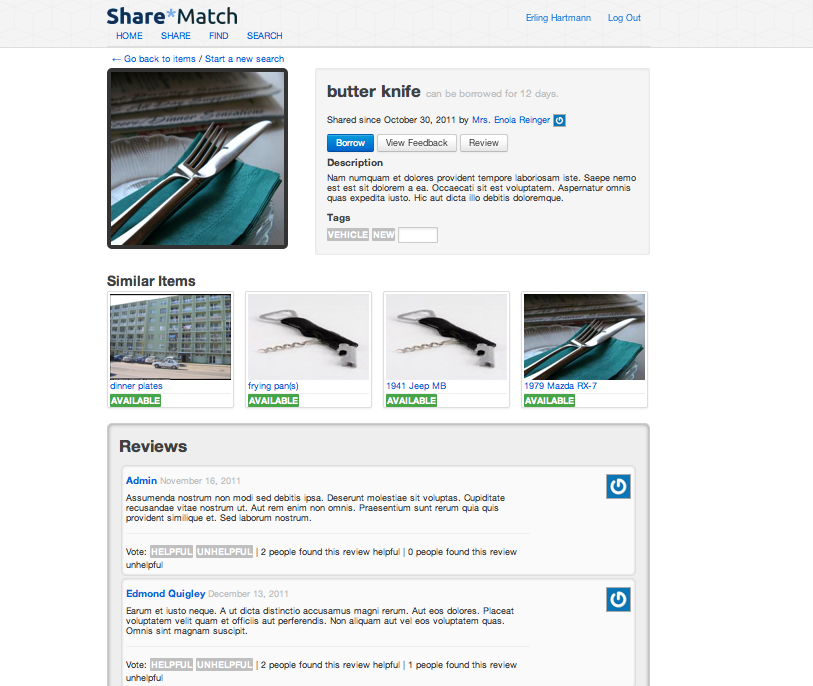
\includegraphics[width=0.4\textwidth]{ItemView.png}
\caption{Item View Page}
\label{fig:ItemView.png}
\end{centering}
\end{figure}
\section{Revisiting the Whole Project}
\subsection{Ian}
For this project, we intentionally included some features to give us a challenge in database design. Because we used an ORM, it was necessary for us to take advantage of this power to build a more complex database. Because of this, there were many different pieces of the database to focus on, each with their own nuanced requirements. This made the project very interesting throughout.
\subsection{Tom}
Our project went by-and-large according to plan. We worked well together, and got most to all features implemented that we wanted to do.
If given unlimited resources, I would like to see our project improve by writing a fuller test suite and switching out the backend to a different ORM, ActiveRecord. The ORM we use, DataMapper, caused us some trouble and perhaps we set it up improperly. Also, the test suite should cover more situations to ensure any future changes are complete and don't affect anything.
Other useful additions to Share*Match include customizable user profiles, automatic friend finding, and integrated authentication with existing networks like Facebook and Twitter. If we made some of these changes, our application is viable to be deployed to the masses.
I would estimate I did about 35%% of the coding myself.

\subsection{Brian}
This project was an excellent opportunity to expand my knowledge of web development.  I had worked in this area a great deal before, but this time we worked from a lower level than before.  This was interesting to see how the frameworks I've used in the past actually implement their underlying helpers as we had to build them ourselves this time.  I think the project was a success.
\section{Team Work}
\subsection{Ian}
For the purposes of collaboration, we used GitHub to manage our code repositories. We made use of the Issues features of GitHub to communicate individual tasks to each other. I found this particularly useful because my schedule did not permit me to communicate directly with Tom and Brian all the time. Instead, we were able to use Issues to decide what we would work on. Furthermore, the application was very modular, which allowed us to split the project up into different pieces for us to work on, preventing versioning conflicts and allowing us to implement our ideas quickly and without collision.
\subsection{Tom}
Brian was the design lead, he did most of the visual design as well as a good portion of the backend. I can't break it into individual features because we all worked on a lot of things. The features that I owned was the entire signup process, including the creating of communities and the display of nearby communities.
We all live together, so team meetings occurred during dinner or at other mutually compatible times. In general it was somewhat difficult to keep everyone on the same page. In general the workflow ended up being Brian taking the larger features (implementing the borrowing methods, review methods, etc.) and the smaller features would trickle down to me. The stuff that trickled down to Ian was primarily bugfixes and small UI improvements.
The division of labor was about as fair as you might assume -- suboptimal but necessitated by the schedules of projects and involvements during the semester.

\subsection{Brian}
Each of the members contributed to this project in a valuable manner.  I couldn't have asked for more from anyone.
\section{Conclusions}
This project met it's goals and was educative for all involved.  The process we used was modern and prepared us well for future work in this area.  We spent a lot of time polishing the project, which probably wasn't all that important in the end.  That is the one thing we would change if doing this over again.
\section{Appendix 1: Installation Manual}
This application follows the standard Ruby web development installation process.  Given a clean install of an operating system, the administrator must install the Ruby programming language. Most Linux distributions will have this in their package repositories, and other operating systems can download it directly from \texttt{http://www.ruby-lang.org/}.  The maintainers of this project however, recommend using RVM, which will automatically keep different Ruby versions separate, including libraries that are insalled. RVM can be found at \texttt{https://rvm.beginrescueend.com/} but will work only for UNIX and Linux operating systems.  

Once Ruby is installed, the administrator must download the source code of this project which can be found at \\\texttt{http://github.com/bis12/eecs341-project}.  Download this into any directory on the local system.  This project requires some non-Ruby gem libraries in order to run properly.  First install \texttt{libsqlite3} and \texttt{imagemagick} from whatever source your operating system normally uses. Then, as with any Ruby project, run \texttt{bundle install} from the top level directory of the project. This will install all of the dependencies of the project.

The application is now ready to run, but has no database.  Before running for the first time,  run \texttt{rake db:rebuild}. This will create all of the databases that you need to run the application.  If this is being run in production mode, just manually add an administrator by running \texttt{tux} in the top level directory and creating a new User with admin privileges.  If this is for development or demonstration purposes, run \texttt{rake db:seed[x]} where \texttt{x} is the number of fake users you want to generate.  This will fill the database with all of the basic objects that interact in this application.  

Once this step is completed the application can be run in one of two modes.  The script to run the application is \texttt{run.sh} and passing it ``production'' will run the application in production mode, whereas an empty string will run it in development mode. Once the server starts and reports that it is listening on the proper ports, go to the url specified and the application will respond.  If the application is seeded with the default seed, there is a user with the email \texttt{admin@sharemat.ch} and password \texttt{password} that will be able to log in.

If this works, the application has been successfully installed!
\section{Appendix 2: Users Manual}
Using ShareMatch should be very easy because it functions the same as any standard web application.  Just access the index page\footnote{which could just be \texttt{http://sharemat.ch} if using the maintainer's install}.  There is a sign up button and log in button in the upper right hand side of the page and find, share, and search links on the upper left. Accessing each of these will allow the user to do the actions specified in the link.  Search is a simple textbox that will search through all of the items to find matches to queries.  Find is merely a listing of items by tags that they have been given, and Share is a form that allows users to add items of their own to ShareMatch.

Once a user navigates to an item that they want to borrow, there is a large blue button on the page that allows the to borrow it.  When clicked, it will alert the owner of the item that a trade should be made, and then the item will go into the possession of the borrower.  The borrow bar then becomes a bar for returning the item.  That process works nearly identically to the borrowing process, except in reverse.

On the page for an item, a user can also review the item, and view other reviews by previous borrowers.   These reviews can be marked helpful or unhelpful.  This all contributes to the community aspect of the project.  

Communities are the most important part of ShareMatch other than the items themselves.  When a user first signs up, they will be stepped through a process of putting in their information, joining a community, and then adding your first item.  The communities will be shown to the user based on the proximity to their stated location.

These are the most important aspects of the process and the rest will be fairly self explanatory.
\section{Appendix 3: Programmer's Manual}
There are a number of classes that make up the application.  The basic architecture of ShareMatch is the MVC pattern, which has models corresponding to database tables, controllers corresponding to RESTful routing endpoints and views that are actually rendered on the web browser.  This design pattern is advantageous because it allows us to separate logically the different parts of the application.  The important models are as follows

\begin{description}
\item[Item] This class holds all of the information about an item that can be borrowed.
\item[User] This is a user of the application. They own and borrow multiple items at a time.
\item[Review] A user reviews an item and it is stored in this object which has multiple joins to Users which indicate how helpful it was.
\item[Tag] Items can be tagged in any number of different fashions to facilitate searching for them.
\item[Community] Users join communities so that only people who are geographically near to one another can share items.
\item[Borrowing]  When a user borrows an item, an entry is made in the Borrowing table, this will include things like whether or not the item was successfully returned.
\end{description}

Those basic objects in addition to a few helpers make up the majority of the model part of our application.  Each one can be interacted with in multiple ways using the different endpoints in the controller layer.


\section*{Notes}
The code for this project can be found at the following location:\\
\texttt{http://github.com/bis12/eecs341-project}
\end{document}
